\documentclass{beamer}
\usepackage[utf8]{inputenc}
\usetheme{Madrid}
\usecolortheme{default}
\usepackage{amsmath,amssymb,amsfonts,amsthm}
\usepackage{txfonts}
\usepackage{tkz-euclide}
\usepackage{listings}
\usepackage{adjustbox}
\usepackage{array}
\usepackage{tabularx}
\usepackage{gvv}
\usepackage{lmodern}
\usepackage{circuitikz}
\usepackage{tikz}
\usepackage{graphicx}
\setbeamertemplate{page number in head/foot}[totalframenumber]
\definecolor{bg}{gray}{0.95}
\lstset{
    language=C,
    basicstyle=\ttfamily\small,
    keywordstyle=\color{blue},
    stringstyle=\color{orange},
    commentstyle=\color{green!60!black},
    numbers=left,
    numberstyle=\tiny\color{gray},
    breaklines=true,
    showstringspaces=false,
}
\title{2.3.8}
\author{Aditya Mishra - EE25BTECH11005}
\date{September 15, 2025}
\begin{document}
\frame{\titlepage}

\begin{frame}{Question}
If $\hat{i} + \hat{j} + \hat{k},\ 2\hat{i} + 5\hat{j},\ 3\hat{i} + 2\hat{j} - 3\hat{k},\ \hat{i} - 6\hat{j} - \hat{k}$ respectively are the position vectors of points $A, B, C,$ and $D$, then find the angle between the straight lines $(\vec{B}-\vec{A})$ and $(\vec{D}-\vec{C})$. Find whether $(\vec{B}-\vec{A})$ and $(\vec{D}-\vec{C})$ are collinear or not.
\end{frame}

\begin{frame}{Given Information}
\[
\vec{A} = \myvec{1\\1\\1},\quad
\vec{B} = \myvec{2\\5\\0},\quad
\vec{C} = \myvec{3\\2\\-3},\quad
\vec{D} = \myvec{1\\-6\\-1}
\]
Direction vectors:
\[
\vec{B}-\vec{A} = \myvec{1\\4\\-1}, \quad
\vec{D}-\vec{C} = \myvec{-2\\-8\\2}
\]
\end{frame}

\begin{frame}{Angle Formula}
The angle $\theta$ between $(\vec{B}-\vec{A})$ and $(\vec{D}-\vec{C})$ is
\begin{align}
\cos \theta = \frac{(\vec{B}-\vec{A})^T (\vec{D}-\vec{C})}
{\|\vec{B}-\vec{A}\| \, \|\vec{D}-\vec{C}\|}
\end{align}
\begin{align}
\theta = \cos^{-1}\left(
\frac{(\vec{B}-\vec{A})^T (\vec{D}-\vec{C})}
{\|\vec{B}-\vec{A}\| \, \|\vec{D}-\vec{C}\|}\right)
\end{align}
\end{frame}

\begin{frame}{Angle Calculation}
\[
(\vec{B}-\vec{A})^T (\vec{D}-\vec{C})
= \myvec{1 & 4 & -1}\myvec{-2 \\ -8 \\ 2}
= -2 - 32 - 2 = -36
\]
\[
\|\vec{B}-\vec{A}\| = \sqrt{1^2 + 4^2 + (-1)^2} = \sqrt{18}
\]
\[
\|\vec{D}-\vec{C}\| = \sqrt{(-2)^2 + (-8)^2 + 2^2} = \sqrt{72}
\]
\[
\cos\theta = \frac{-36}{\sqrt{18}\,\sqrt{72}} = -1
\]
\[
\theta = \cos^{-1}(-1) = 180^\circ
\]
\end{frame}

\begin{frame}{Collinearity using Rank}
For collinearity, form the matrix
\[
M = \myvec{1 & 4 & -1 \\ -2 & -8 & 2}
\]
Row-reducing:
\[
R_2 \to R_2 + 2R_1 \implies \myvec{1 & 4 & -1 \\ 0 & 0 & 0}
\]
\[
\text{rank}(M) = 1
\]
Thus, $(\vec{B}-\vec{A})$ and $(\vec{D}-\vec{C})$ are collinear.  
Since $\theta = 180^\circ$, they are anti-parallel.
\end{frame}

\begin{frame}{Plot}
\begin{figure}
    \centering
    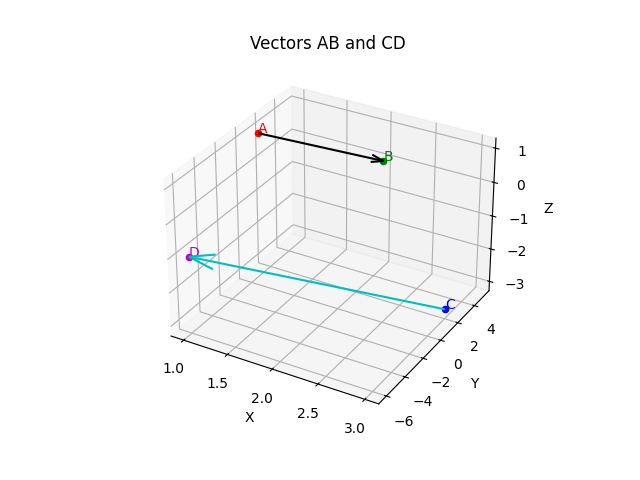
\includegraphics[width=0.8\columnwidth]{Figs/Figure.png}
\end{figure}
\end{frame}

\begin{frame}{Codes}
\centering
For Codes, refer to the URL below:  
\url{https://github.com/Aditya-Mishra11005/ee1030-2025/tree/main/ee25btech11005/matgeo/2.3.8/Codes}
\end{frame}

\end{document}

